\section{Introduction}
\label{sec:introduction}
Systems for complex event processing (CEP) continuously evaluate a set of
queries over streams of event
data~\cite{DBLP:journals/csur/CugolaM12,DBLP:journals/vldb/GiatrakosAADG20}. As
such, they facilitate the recognition of situations of interest that
materialize as event patterns, thereby enabling reactive and proactive
applications in various domains, including, for instance,
supply chain management~\cite{DBLP:journals/cii/KonovalenkoL19}, urban
transportation~\cite{DBLP:conf/edbt/ArtikisWSBLPBMKMGMGK14}, and
computational finance~\cite{DBLP:journals/computer/ChandramouliAGSR10}.
CEP systems provide a rich model for the
specification of
event queries~\cite{DBLP:conf/debs/ArtikisMUVW17}. Queries typically define
conditions over the attribute values of events to establish their relevance
for a pattern and to correlate them; and they impose constraints on the
ordering of events and their occurrence within a certain window over the
stream.
While event queries enable a comprehensive characterization of a situation of
interest, their specification is challenging in practice. Domain experts may
have a basic understanding of factors that contribute to a
situation that shall be detected by a query, but typically lack full knowledge
about the specific event patterns, in particular in predictive
applications~\cite{DBLP:conf/debs/EngelEF12,DBLP:conf/debs/SejdovicHRS16}.
Here, the occurrence of a
situation (e.g., a delay in a supply chain or a
fraudulent
transaction) is anticipated in order to prevent or mitigate it.
\begin{wrapfigure}{r}{.5\columnwidth}
	\centering
	\vspace{-1em}
	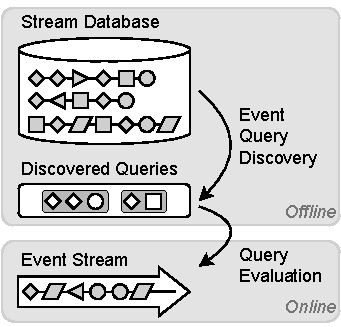
\includegraphics[width=0.5\columnwidth]{img/overview.drawio.pdf}
	\vspace{-2.0em}
	\caption{The general setting.}
	\label{fig:overview}
	\vspace{-1em}
\end{wrapfigure}
To support the specification of event queries, approaches for automated query
discovery have been proposed~\cite{icep,ilminer}. They assume that a database
of finite, historic (sub-)streams, each including at least one
materialization of
the situation, is available, \change{see \autoref{fig:overview}.
Algorithmically discovering queries that match given streams
can generalize historic observations. These resulting queries can
then be reviewed and refined by domain experts before being evaluated
over an event stream to detect future occurrences of the situation of interest.}
Unlike machine learning approaches for pattern detection, the discovery of
event queries provides a traceable and
explainable characterization of a situation of interest.
Solving the problem of event query discovery is computationally hard, though.
The search space of candidate queries grows exponentially in
the query length and the size of the domain of the payload data. Existing
discovery approaches~\cite{icep,ilminer} explore this
space in \emph{one} specific way, which may be suitable for one
database, but leads to intractability for another one. Yet, the assumptions on
the database that motivate the taken design choices are implicit, so that it is
unclear for which database an algorithm can be expected to work.
In this paper, we argue for the systematic design of algorithms for
event query discovery. We aim to answer the following question:
\begin{enumerate}[label=(\roman*),left=0pt,nosep]
\item \emph{What are the design choices in query discovery?}
\item \emph{How to choose a design for a given database?}
\item \emph{How to provide feedback on the algorithmic performance?}
\end{enumerate}
We address these questions through three contributions that we summarize,
along
with the paper structure following a problem formalization
(\autoref{sec:problem}), as follows:
\begin{enumerate}[left=0pt,nosep]
\item We present \sys{} (\autoref{sec:framework})
as a framework
for the design of algorithms for event query
discovery. It captures a set of fundamental design
choices to define discovery algorithms.
\item We instantiate the framework to derive four
discovery algorithms
(\autoref{sec:algos}). They all provide correct
and complete results, yet they differ in their exploration of the space of
candidate queries.
\item We provide means to guide event query discovery
(\autoref{sec:instantiation}). First, we show how to choose among our
algorithms based on a few essential properties of a given stream database.
Second, we provide hints on how to resolve intractability or ineffectiveness of
discovery based on abstractions of the events' payload data.
\end{enumerate}
We evaluated our techniques in experiments using simulated and
real-world data (\autoref{sec:evaluation}). Our results illustrate that the
algorithms designed as part of
the \sys{} framework are indeed tailored to databases that show certain
properties. They solve the query discovery problem
several orders of magnitude faster than existing approaches,
with runtimes that are comparable to
strategies that approximate the result.
We close with a review of related work (\autoref{sec:related_work}) and
conclusions (\autoref{sec:conclusions}).